\documentclass[../../Thesis.tex]{subfiles}
\begin{document}

\header{Experiment setup}
We used the following pipeline to collect the performance metrics for the categorization task:
\begin{enumerate}
\item{Create embeddings}
\item{Filter articles}
\item{Create training and validation set}
\item{Create journal embeddings}
\item{Categorize validation articles}
\item{Calculate performance metrics}
\end{enumerate}

\subheader{Create embeddings}
For this research, we used word-embeddings (created using the word2vec model) and TF-IDF embeddings. The word-embeddings were created with the word2vec model from PySparks MlLib library\cite{PysparkMlLib}. The embeddings were pre-trained and have a vector size of 300, which is an industry default. The TF-IDF embeddings were created with the TF-IDF model from pyspark's MlLib library\cite{PysparkMlLib}, in combination with a token hasher (HashingTF) from the same library. We used multiple hashing dimensions and multiple vocabulary sizes. Since the TF-IDF uses the output of the term hasher, the TF-IDF model produces the same dimensions. We will denote the tfidf sets as vocabulary size/hashing size. All of our sets, both embedding and TF-IDF, use tokenized texts.
\subsubheader{Tokenization}
== TODO ==
\subsubheader{TF-IDF selection}
To limit computational expenses, we used only the top performing which can reasonably be kept in RAM. The plot displays the ranking \& size for the 1000/1000, 4000/4000, 7000/7000 and 10.000/10.000 sets respectively.\\
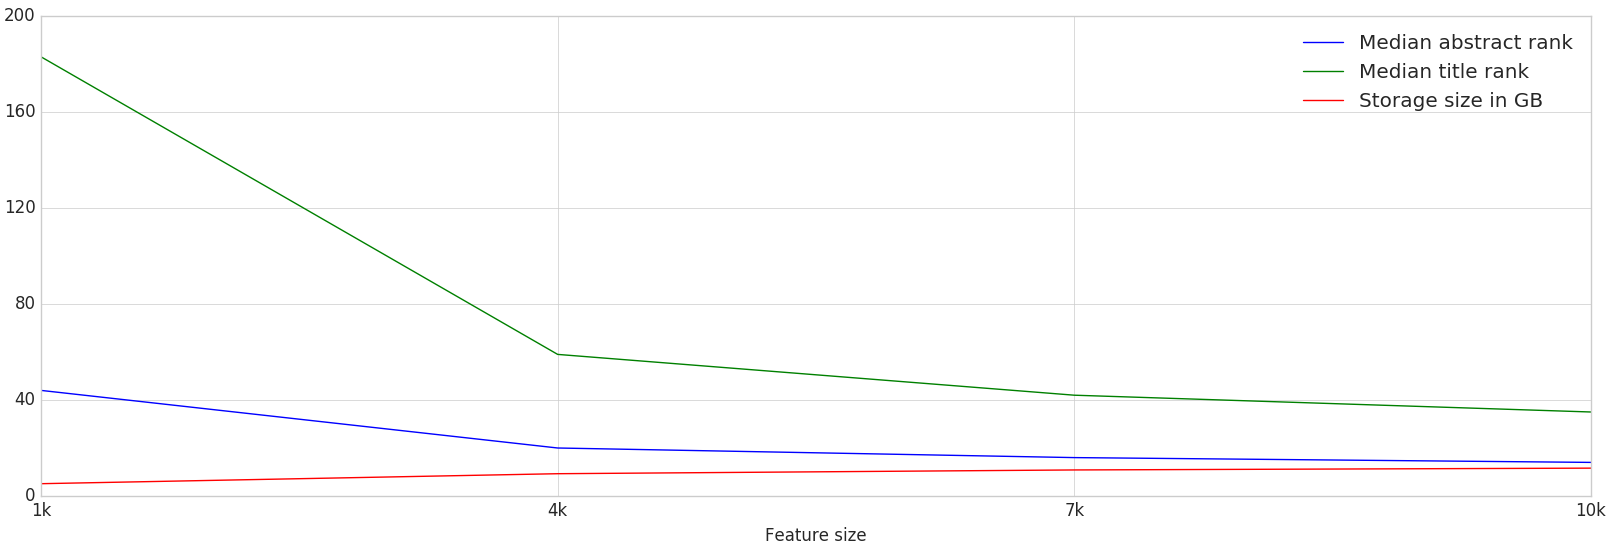
\includegraphics[width=6in]{Plots/tfidf_selection_plot}\\
The plot show the median abstract \& title rank and the storage size in Gigabytes (1024 based) plotted over feature size, which is equal to the hashing size for these sets. The plot shows that both title and abstract are stagnating, while the memory usage is, slowly, going up. At a feature size of 10.000, we have a storage size of 11.6GB. Given this size and the stagnation of the rankings, we chose to use the 10.000/10.000 feature size tfidf vectors, we furthermore used the 10.000/5000 set and the 5000/5000 set for comparison.

\subsubheader{Embeddings}
We have made use of multiple embedding sets for this research. All sets share the same (default) embedding and have been (uniquely) modified. For this research we have used the following embedding sets:
\begin{enumerate}
\item{Default embedding}
\subitem{The embedding as generated by word2vec, without further enhancements.}
\item{TF-IDF embedding}
\subitem{The embedding as generated by the word2vec, multiplied by their tfidf weights to embed word priorities. We use this enhancement to give the embeddings more information about the corpus.}
\item{10K TF-IDF Embedding}
\subitem{The embedding as generated by the word2vec, filtered on the top 10.000 most common words, multiplied by their tfidf weights.\\We use this enhancement to try to filter out possible noise created by lots of words with few occurrences.}
\item{5K TF-IDF Embedding}
\subitem{The embedding as generated by the word2vec, filtered on the top 5.000 most common words, multiplied by their tfidf weights.\\We use this enhancement to cancel out the noise caused be rare words more aggressively}
\item{1K 6K TF-IDF Embedding}
\subitem{The embeddings as generated by the word2vec, filtered on the top top 1.000 till top 5.000 most common words, multiplied by their tfidf weights.\\We use this enhancement to ignore the top 1.000 most common words, which are most likely generic words, since they occur often. And to cancel out the rare-words, by cutting off all words after 6K. This gives us a set of 5K words.}
\end{enumerate}
  
\subheader{Filter articles}
We create our initial set of articles by collecting all articles from the journals that were published in the year 2017, and have at least 200 publications in 2017. This reduces the journal set to $3,759$ thousand journals, resulting in a set of $1,391,543$ million articles ().
\subheader{Create training and validation set}
We split our initial set  $80\%$ - $20\%$,. We use the $80\%$ set as the training set for the journal representations, and the $20\%$ set as the validation set for the journal representations.
\subheader{Create journal embeddings}
From our training set we create the journal embeddings by averaging all title embeddings as the journal title embedding, and by averaging all abstract embeddings as the journal abstract embedding. We also normalized both embeddings. 
\subheader{Categorize validation articles}
To categorize the articles, we calculate the distance between the title- and abstract embedding of each article, from the validation set, to the title- and abstract embedding of each journal. To calculate the distance, we use cosine similarity (as provided by the SciPy library\cite{SciPy}). During this process we keep track of:
\begin{itemize}
\item{Title-based-rank of the actual journal}
\item{Abstract-based-rank of the actual journal}
\item{Best scored journal on the abstract similarity}
\item{Best scored journal on the title similarity}
\item{Abstract similarity between the actual journal and the article}
\item{Title similarity between the actual journal and the article}
\end{itemize}
\subheader{Performance measurement}
We use multiple metrics to indicate the performance of the embeddings on a categorization task. These metrics are:
\begin{enumerate}
\item{F1-score}
\item{Median \& average rank}
\item{Rank distribution}
\end{enumerate}
\subsubheader{F1-score}
We define the positive \& negative metrics as follows:\\
\begin{jumpin}
$True Positive = $ Articles that are correctly matched to the current journal\\
$False Positive = $ Articles that are incorrectly matched to other journals\\
$False Negative = $ Articles that are incorrectly matched to the current journal\\
\end{jumpin}
We used these metrics to calculate the Recall, Precision \& F1 as follows:\\
\begin{jumpin}
$Recall = \dfrac{True Positive}{True Positive + False Negative}$\vspace{0.1in}\\
$Precision = \dfrac{True Positive}{True Positive + False Positive}$\vspace{0.1in}\\
$F1 = \dfrac{2 * Precision * Recall}{Precision + Recall}$
\end{jumpin}
\subsubheader{Median \& average rank}
We use the median rank to indicate around which rank the 'standard' article would be ranked, based on its title or abstract. We do this by taking the median of the respective rank from each article. This gives us an indication of the behaviour of most articles in our validation set. This median rank (mostly) ignores the outliers, we therefore also use the average rank, which gives a more global indication, although this rank may be over-influenced by some outliers.
\subsubheader{Rank distribution}
To further analyse the ranking results, we plot the rank distribution to get an indication of the ranking-landscape. We limit ourselves to the following categories: 1 (absolute hits), top-10, top-20, top-30, top-40, top-50,  top-100 and 100+. 
\end{document}


